%-------------------------------------------------------------------------
% q-info-S1-conclusion.tex
%-------------------------------------------------------------------------
\def\reseau{%
\begin{picture}(8.5,4.5)        
\put(1,2.5){\makebox(0,0){$\bullet$}}
\put(0.7,2.5){\makebox(0,0){ s}} 
\put(1.75,3){\makebox(0,0){\tiny 3}}  % s-a 
\put(1.75,2){\makebox(0,0){\tiny 4}} % s-d
\put(2.75,2.5){\makebox(0,0){\tiny 5}}  % a-d 
\put(3.5,3.75){\makebox(0,0){\tiny 4}}  % a-b
\put(4.75,2.5){\makebox(0,0){\tiny 5}}  % b-e
\put(3.5,1.25){\makebox(0,0){\tiny 2}}  % d-e
\put(5.5,1.25){\makebox(0,0){\tiny 4}}  % e-f
\put(7.25,2){\makebox(0,0){\tiny 3}}  % f-g
\put(5.5,3.75){\makebox(0,0){\tiny 4}}  % b-c
\put(1,2.5){\line(1,1){1.5}}
\put(1,2.5){\line(1,-1){1.5}}
\put(2.5,4){\makebox(0,0){$\bullet$}}
\put(2.5,4.3){\makebox(0,0){ a}}
\put(2.5,1){\makebox(0,0){$\bullet$}}
\put(2.5,0.75){\makebox(0,0){ d}} 
\put(2.5,4){\line(1,0){4}}
\put(2.5,1){\line(1,0){4}}
\put(4.5,1){\makebox(0,0){$\bullet$}} 
\put(4.5,0.75){\makebox(0,0){ e}}
\put(6.5,1){\makebox(0,0){$\bullet$}} 
\put(6.5,0.75){\makebox(0,0){ f}}
\put(6.5,1){\line(1,1){1.5}}
\put(8,2.5){\makebox(0,0){$\bullet$}} 
\put(8.2,2.5){\makebox(0,0){ g}} 
\put(4.5,4){\makebox(0,0){$\bullet$}} 
\put(4.5,4.3){\makebox(0,0){ b}}
\put(6.5,4){\makebox(0,0){$\bullet$}}
\put(6.5,4.3){\makebox(0,0){ c}} 
\put(2.5,4){\line(0,-1){3}} 
\put(4.5,4){\line(0,-1){3}}
%\put(4.5,0){\makebox(0,0){\normalsize r\'eseau routier}} 
\end{picture}}

\noindent\begin{minipage}{10cm}
\begin{description}
\item[Objectif :] mettre en \oe uvre l'ensemble des notions abordées dans ce document
	à travers l'exemple général de la recherche d'un chemin dans un graphe.
\end{description}
\end{minipage}
\hfill
\begin{minipage}{4cm}
Graphe\\
\fbox{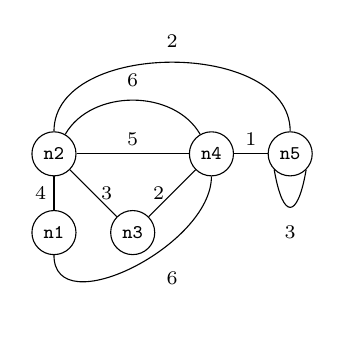
\begin{tikzpicture}[scale=1]\scriptsize
\node[draw,circle] (A) at (0,0) {\texttt{n1}};
\node[draw,circle] (B) at (0,1) {\texttt{n2}};
\node[draw,circle] (C) at (1,0) {\texttt{n3}};
\node[draw,circle] (D) at (2,1) {\texttt{n4}};
\node[draw,circle] (E) at (3,1) {\texttt{n5}};
\draw (A) -- (B);
\draw (0,0.5) node[left] {4};
\draw (B) -- (C);
\draw (0.5,0.5) node[right] {3};
\draw (A) to[out=-90,in=-90] (D);
\draw (B) to[out=60,in=120] (D);
\draw (B) -- (D);
\draw (C) -- (D);
\draw (1.5,0.5) node[left] {2};
\draw (1,1) node[above] {5};
\draw (1.5,-0.4) node[below] {6};
\draw (1,1.75) node[above] {6};
\draw (D) -- (E);
\draw (2.5,1) node[above] {1};
\draw (B) to[out=90,in=90] (E);
\draw (1.5,2.25) node[above] {2};
\coordinate[shift={(0mm,-1cm)}] (n) at (E.south);
\draw[rounded corners=30pt] (E.south west) -- (n) -- (E.south east);
\draw (3,0) node {3};
\end{tikzpicture}}
\end{minipage}

%-------------------------------------------------------------------------
\subsection{Exemple}
%-------------------------------------------------------------------------

\paragraph{Enoncé :}
Dans le premier exemple introductif (section \ref{sec:algo}, exemple \ref{ex:restaurant} 
page \pageref{ex:restaurant} : «~aller au restaurant~»)
un touriste devait rejoindre un restaurant depuis son hôtel.
On peut, en première approximation, assimiler le plan de la ville à un graphe dont 
les n\oe uds ($\bullet$) sont les carrefours et les arcs ($\rule[0.5ex]{1cm}{1pt}$)
les tronçons de rues entre deux carrefours, comme suggéré sur la figure ci-dessous. 
Le problème ainsi transposé devient la recherche d'un chemin d'un carrefour à un autre
au sein d'un réseau urbain connu sans passer deux fois par le même carrefour.
\vspace*{3mm}

%C'est ce problème plus abstrait qui est traité dans cette section car il met en \oe uvre l'ensemble des notions abordées précédemment. Une fois résolu, nous pourrons l'appliquer
%à la recherche d'un chemin dans un réseau routier et l'étendre à titre d'exemples à 
%des applications «~ludiques~».

\noindent\begin{minipage}{7cm}
\includegraphics[width=7cm]{plan.pdf}
\end{minipage}
\hfill
\begin{minipage}{7cm}
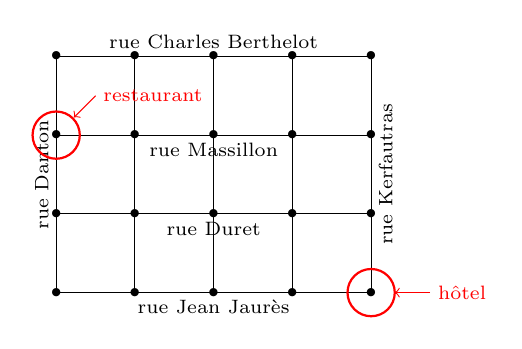
\begin{tikzpicture}[scale=1]\scriptsize
\draw (0,0) -- (4,0) node[midway,below] {rue Jean Jaurès};
\draw (0,1) -- (4,1) node[midway,below] {rue Duret};
\draw (0,2) -- (4,2) node[midway,below] {rue Massillon};
\draw (0,3) -- (4,3) node[midway,above] {rue Charles Berthelot};
\draw (0,0) -- (0,3) node[midway,above,rotate=90] {rue Danton};
\draw (1,0) -- (1,3);
\draw (2,0) -- (2,3);
\draw (3,0) -- (3,3);
\draw (4,0) -- (4,3) node[midway,below,rotate=90] {rue Kerfautras};
\foreach \x in {0,1,...,4} \foreach \y in {0,1,2,3} \draw (\x,\y) node {$\bullet$};
\draw[color=red,thick] (0,2) circle(0.3);
\draw[color=red,->] (0.5,2.5) node[right] {restaurant} -- (0.225,2.225);
\draw[color=red,thick] (4,0) circle(0.3);
\draw[color=red,->] (4.75,0) node[right] {hôtel} -- (4.3,0);
\end{tikzpicture}
\end{minipage}
\vspace*{3mm}

\paragraph{Méthode :} Rechercher un chemin entre deux n\oe uds d'un graphe sans passer 
deux fois par le même n\oe ud revient à parcourir un arbre de recherche comme le montre 
la figure ci-dessous. Dans le réseau routier (à gauche de la figure), on cherche à se rendre de 
\texttt{s} à \texttt{g}, ce qui revient à parcourir l'arbre de recherche (à droite de la figure)
dans lequel on observe qu'il y a 4 chemins différents pour se rendre de \texttt{s} à \texttt{g} :
\texttt{[s,a,b,e,f,g]} de 19 km, \texttt{[s,a,d,e,f,g]} (17 km), \texttt{[s,d,a,b,e,f,g]} (25 km)
et \texttt{[s,d,e,f,g]} (13 km), les autres chemins étant des impasses dans ce contexte. 
\vspace*{3mm}

\noindent\begin{minipage}{5.25cm}
\setlength\unitlength{0.6cm}\footnotesize
\reseau
\end{minipage}
\hfill$\longrightarrow$\hfill
\begin{minipage}{8.75cm}
\setlength{\unitlength}{0.6cm}\footnotesize
\begin{picture}(14,6)%\color{lightgray}
%\put(7,7){\makebox(0,1){\LARGE Pour aller de {s} \`a {g}}} 
\put(7,6){\makebox(0,0){$\bullet$}}
\put(7,6.3){\makebox(0,0){s}}
\put(7,6){\line(-4,-1){4}}
\put(7,6){\line(4,-1){4}} 
\put(3,5.3){\makebox(0,0){a}}
\put(3,5){\makebox(0,0){$\bullet$}}
\put(11,5.3){\makebox(0,0){d}}
\put(11,5){\makebox(0,0){$\bullet$}}
\put(3,5){\line(-2,-1){2}}
\put(3,5){\line(2,-1){2}}
\put(1,4.3){\makebox(0,0){b}}
\put(1,4){\makebox(0,0){$\bullet$}}
\put(5,4.3){\makebox(0,0){d}}
\put(5,4){\makebox(0,0){$\bullet$}}
\put(1,4){\line(-1,-1){1}}
\put(1,4){\line(1,-1){1}}   
\put(0,2.7){\makebox(0,0){c}}
\put(0,3){\makebox(0,0){$\bullet$}}
\put(2,3.3){\makebox(0,0){e}}
\put(2,3){\makebox(0,0){$\bullet$}}
\put(2,3){\line(-1,-1){1}}
\put(2,3){\line(1,-1){1}}    
\put(1,1.7){\makebox(0,0){d}}
\put(1,2){\makebox(0,0){$\bullet$}}
\put(3,2.3){\makebox(0,0){f}}
\put(3,2){\makebox(0,0){$\bullet$}}
\put(3,2){\line(0,-1){1}}
\put(3,0.7){\makebox(0,0){g}} 
\put(3,1){\makebox(0,0){$\bullet$}}
\put(5,4){\line(0,-1){1}}
\put(5.3,3.1){\makebox(0,0){e}}
\put(5,3){\makebox(0,0){$\bullet$}}
\put(5,3){\line(-1,-1){1}}
\put(5,3){\line(1,-1){1}}   
\put(4,2.3){\makebox(0,0){b}}
\put(4,2){\makebox(0,0){$\bullet$}}
\put(6,2.3){\makebox(0,0){f}}
\put(6,2){\makebox(0,0){$\bullet$}}
\put(4,2){\line(0,-1){1}}
\put(4,0.7){\makebox(0,0){c}}
\put(4,1){\makebox(0,0){$\bullet$}}
\put(6,2){\line(0,-1){1}}
\put(6,0.7){\makebox(0,0){g}}
\put(6,1){\makebox(0,0){$\bullet$}}
\put(11,5){\line(-2,-1){2}}
\put(9,4.3){\makebox(0,0){a}}
\put(9,4){\makebox(0,0){$\bullet$}}
\put(9,4){\line(0,-1){1}}
\put(9.3,3.1){\makebox(0,0){b}}
\put(9,3){\makebox(0,0){$\bullet$}}
\put(9,3){\line(-1,-1){1}}
\put(9,3){\line(1,-1){1}}   
\put(8,1.7){\makebox(0,0){c}}
\put(8,2){\makebox(0,0){$\bullet$}}
\put(10,2.3){\makebox(0,0){e}}
\put(10,2){\makebox(0,0){$\bullet$}}
\put(10,2){\line(0,-1){1}}
\put(10.3,1){\makebox(0,0){f}}
\put(10,1){\makebox(0,0){$\bullet$}}
\put(10,1){\line(0,-1){1}}
\put(10,-0.3){\makebox(0,0){g}} 
\put(10,0){\makebox(0,0){$\bullet$}} 
\put(11,5){\line(2,-1){2}}
\put(13,4.3){\makebox(0,0){e}}
\put(13,4){\makebox(0,0){$\bullet$}}
\put(13,4){\line(-1,-1){1}}
\put(13,4){\line(1,-1){1}}   
\put(12,3.3){\makebox(0,0){b}}
\put(12,3){\makebox(0,0){$\bullet$}}
\put(12,3){\line(-1,-1){1}}
\put(12,3){\line(1,-1){1}}   
\put(14,3.3){\makebox(0,0){f}}
\put(14,3){\makebox(0,0){$\bullet$}}
\put(14,3){\line(0,-1){1}}
\put(11,1.7){\makebox(0,0){a}}
\put(11,2){\makebox(0,0){$\bullet$}}
\put(13,1.7){\makebox(0,0){c}}  
\put(13,2){\makebox(0,0){$\bullet$}}
\put(14,1.7){\makebox(0,0){g}}
\put(14,2){\makebox(0,0){$\bullet$}}
%\color{orange}
%\thicklines
\put(7,6){\line(-4,-1){4}}
\put(3,5){\line(-2,-1){2}}
\put(1,4){\line(1,-1){1}}
\put(2,3){\line(1,-1){1}}
\put(3,2){\line(0,-1){1}}
\put(3,0){\makebox(0,0){(19)}}
\put(3,5){\line(2,-1){2}}
\put(5,4){\line(0,-1){1}}
\put(5,3){\line(1,-1){1}}
\put(6,2){\line(0,-1){1}}
\put(6,0){\makebox(0,0){(17)}}
\put(7,6){\line(4,-1){4}} 
\put(11,5){\line(-2,-1){2}}
\put(9,4){\line(0,-1){1}}
\put(9,3){\line(1,-1){1}}   
\put(10,2){\line(0,-1){1}}
\put(10,1){\line(0,-1){1}}
\put(10,-1){\makebox(0,0){(25)}}
\put(11,5){\line(2,-1){2}}
\put(13,4){\line(1,-1){1}}   
\put(14,3){\line(0,-1){1}}
\put(14,1){\makebox(0,0){(13)}}
\end{picture}
\end{minipage}
\newpage

On utilisera donc des méthodes de parcours d'arbre pour ce type de recherche
(recherche en profondeur, en largeur ou du meilleur chemin).
Dans un premier temps, nous introduirons un certain nombre de notions 
(piles, files, graphes) qui seront utiles à la recherche d'un chemin 
dans un graphe.

%-------------------------------------------------------------------------
\subsubsection{Piles et files}\label{subsec:pile}
%-------------------------------------------------------------------------

\noindent\begin{minipage}[t]{7.7cm}
{Pile : structure \textsc{Lifo}}\\
\fbox{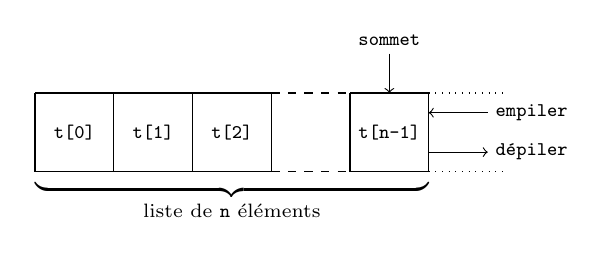
\begin{tikzpicture}[scale=1]\scriptsize
\draw (0,0) -- (3,0);
\draw (0,1) -- (3,1);
\draw[dashed] (3,0) -- (4,0);
\draw[dashed] (3,1) -- (4,1);
\draw (4,0) -- (5,0);
\draw (4,1) -- (5,1);
\draw[dotted] (5,0) -- (6,0);
\draw[dotted] (5,1) -- (6,1);
\draw (0,0) -- (0,1);
\draw (0.5,0.5) node {\texttt{t[0]}};
\draw (1,0) -- (1,1);
\draw (1.5,0.5) node {\texttt{t[1]}};
\draw (2,0) -- (2,1);
\draw (2.5,0.5) node {\texttt{t[2]}};
\draw (3,0) -- (3,1);
\draw (4,0) -- (4,1);
\draw (5,0) -- (5,1);
\draw (4.5,0.5) node {\texttt{t[n-1]}};
\draw (4.5,1.5) node[above] {\texttt{sommet}};
\draw[->] (4.5,1.5) -- (4.5,1);
\draw (5.75,0.75) node[right] {\texttt{empiler}};
\draw (5.75,0.25) node[right] {\texttt{dépiler}};
\draw[->] (5.75,0.75) -- (5,0.75);
\draw[->] (5,0.25) -- (5.75,0.25);
\draw (2.5,0) node[below] {$\underbrace{\makebox[5cm]{}}_{\mbox{liste de \texttt{n} éléments}}$};
\end{tikzpicture}}
\end{minipage}
\hfill
\begin{minipage}[t]{8cm}
{File : structure \textsc{Fifo}}\\
\fbox{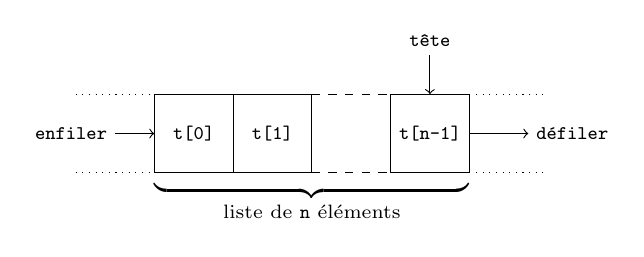
\begin{tikzpicture}[scale=1]\scriptsize
\draw[dotted] (0,0) -- (1,0);
\draw[dotted] (0,1) -- (1,1);
\draw (1,0) -- (3,0);
\draw (1,1) -- (3,1);
\draw[dashed] (3,0) -- (4,0);
\draw[dashed] (3,1) -- (4,1);
\draw (4,0) -- (5,0);
\draw (4,1) -- (5,1);
\draw[dotted] (5,0) -- (6,0);
\draw[dotted] (5,1) -- (6,1);
\draw (1,0) -- (1,1);
\draw (1.5,0.5) node {\texttt{t[0]}};
\draw (2,0) -- (2,1);
\draw (2.5,0.5) node {\texttt{t[1]}};
\draw (3,0) -- (3,1);
\draw (4,0) -- (4,1);
\draw (5,0) -- (5,1);
\draw (4.5,0.5) node {\texttt{t[n-1]}};
\draw (4.5,1.5) node[above] {\texttt{tête}};
\draw[->] (4.5,1.5) -- (4.5,1);
\draw (0.5,0.5) node[left] {\texttt{enfiler}};
\draw[->] (0.5,0.5) -- (1,0.5);
\draw (5.75,0.5) node[right] {\texttt{défiler}};
\draw[->] (5,0.5) -- (5.75,0.5);
\draw (3,0) node[below] {$\underbrace{\makebox[4cm]{}}_{\mbox{liste de \texttt{n} éléments}}$};
\end{tikzpicture}}
\end{minipage}

\begin{question}[« tout en un » : piles]
Une pile (structure \textsc{Lifo} : \emph{last in, first out}) sera représentée ici par une liste. On empilera et dépilera en fin de liste.
\begin{enumerate}
\item Définir la fonction \texttt{pileVide} qui teste si une pile \texttt{p}
	est vide (\texttt{True}) ou non (\texttt{False}).

\noindent\begin{minipage}[t]{6cm}\tt\footnotesize
\begin{Verbatim}
>>> pileVide([])
True
\end{Verbatim}
\end{minipage}
\hfill
\begin{minipage}[t]{6cm}\tt\footnotesize
\begin{Verbatim}
>>> pileVide([1,2,3])
False
\end{Verbatim}
\end{minipage}
\vspace*{2mm}
	
\item Définir la fonction \texttt{sommet} qui retourne le sommet \texttt{s}
	d'une pile \texttt{p} non vide.

\noindent\begin{minipage}[t]{6cm}\tt\footnotesize
\begin{Verbatim}
>>> sommet([1,2,3])
3
\end{Verbatim}
\end{minipage}
\hfill
\begin{minipage}[t]{6cm}\tt\footnotesize
\begin{Verbatim}
>>> sommet([])
    assert not pileVide(p)
AssertionError
\end{Verbatim}
\end{minipage}
\vspace*{2mm}
	
\item Définir la fonction \texttt{empiler} qui empile un élément \texttt{e}
	au sommet d'une pile \texttt{p}.

\noindent\begin{minipage}[t]{6cm}\tt\footnotesize
\begin{Verbatim}
>>> p = [1,2,3]
>>> empiler(p,7)
>>> p
[1, 2, 3, 7]
\end{Verbatim}
\end{minipage}
\hfill
\begin{minipage}[t]{6cm}\tt\footnotesize
\begin{Verbatim}
>>> p = []
>>> empiler(p,7)
>>> p
[7]
\end{Verbatim}
\end{minipage}
\vspace*{2mm}
	
\item Définir la fonction \texttt{depiler} qui retourne le sommet \texttt{s}
	d'une pile \texttt{p} non vide après l'avoir dépilée.

\noindent\begin{minipage}[t]{6cm}\tt\footnotesize
\begin{Verbatim}
>>> p = [1,2,3]
>>> depiler(p)
3
>>> depiler(p)
2
\end{Verbatim}
\end{minipage}
\hfill
\begin{minipage}[t]{6cm}\tt\footnotesize
\begin{Verbatim}
>>> depiler(p)
1
>>> depiler(p)
    assert not pileVide(p)
AssertionError
\end{Verbatim}
\end{minipage}
\vspace*{2mm}

\end{enumerate}

\end{question}

\begin{question}[« tout en un »  : files] 
Une file (structure \textsc{Fifo} : \emph{first in, first out}) sera représentée ici par une liste. On enfilera en début de liste
et défilera en fin de liste.
\begin{enumerate}
\item Définir la fonction \texttt{fileVide} qui teste si une file \texttt{f}
	est vide (\texttt{True}) ou non (\texttt{False}).

\noindent\begin{minipage}[t]{6cm}\tt\footnotesize
\begin{Verbatim}
>>> fileVide([])
True
\end{Verbatim}
\end{minipage}
\hfill
\begin{minipage}[t]{6cm}\tt\footnotesize
\begin{Verbatim}
>>> fileVide([1,2,3])
False
\end{Verbatim}
\end{minipage}
\vspace*{2mm}
	
\item Définir la fonction \texttt{tete} qui retourne la tête \texttt{t}
	d'une pile \texttt{f} non vide.

\noindent\begin{minipage}[t]{6cm}\tt\footnotesize
\begin{Verbatim}
>>> tete([1,2,3])
3
\end{Verbatim}
\end{minipage}
\hfill
\begin{minipage}[t]{6cm}\tt\footnotesize
\begin{Verbatim}
>>> tete([])
    assert not fileVide(f)
AssertionError
\end{Verbatim}
\end{minipage}
\vspace*{2mm}
	
\item Définir la fonction \texttt{enfiler} qui enfile un élément \texttt{e}
	dans une une file \texttt{f}.

\noindent\begin{minipage}[t]{6cm}\tt\footnotesize
\begin{Verbatim}
>>> f = [1,2,3]
>>> enfiler(f,7)
>>> f
[7, 1, 2, 3]
\end{Verbatim}
\end{minipage}
\hfill
\begin{minipage}[t]{6cm}\tt\footnotesize
\begin{Verbatim}
>>> f = []
>>> enfiler(f,7)
>>> f
[7]
\end{Verbatim}
\end{minipage}
\vspace*{2mm}
	
\item Définir la fonction \texttt{defiler} qui retourne la tête \texttt{t}
	d'une file \texttt{f} non vide après l'avoir défilée.

\noindent\begin{minipage}[t]{6cm}\tt\footnotesize
\begin{Verbatim}
>>> f = [1,2,3]
>>> defiler(f)
3
>>> defiler(f)
2
\end{Verbatim}
\end{minipage}
\hfill
\begin{minipage}[t]{6cm}\tt\footnotesize
\begin{Verbatim}
>>> defiler(f)
1
>>> defiler(f)
    assert not fileVide(f)
AssertionError
\end{Verbatim}
\end{minipage}
\vspace*{2mm}

\end{enumerate}

\end{question}

%-------------------------------------------------------------------------
\subsubsection{Graphes}
%-------------------------------------------------------------------------

\noindent
\begin{minipage}{10cm}
Un graphe peut être vu comme un ensemble de n\oe uds reliés 
entre eux par des arcs comme dans l'exemple ci-contre.
Les n\oe uds et les arcs peuvent être étiquetés. Pour les arcs, l'étiquette
est appelée le poids de l'arc : l'arc qui relie ci-contre les n\oe uds 
\texttt{n1} et \texttt{n4} a un poids de \texttt{6}.
Un graphe peut avoir des arcs multiples : plusieurs arcs différents relient 
la même paire de n\oe uds comme c'est le cas pour les n\oe uds \texttt{n2}
et \texttt{n4} ci-contre. Un arc peut ne relier qu'un n\oe ud à lui-même
comme la boucle sur le n\oe ud \texttt{n5} avec un poids de \texttt{3}. 
\end{minipage}
\hfill
\begin{minipage}{4cm}
Graphe\\
\fbox{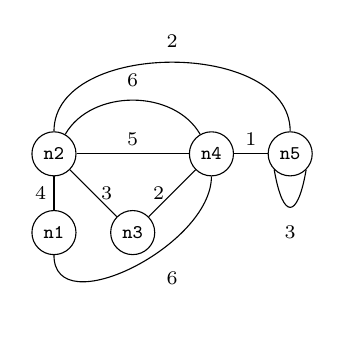
\begin{tikzpicture}[scale=1]\scriptsize
\node[draw,circle] (A) at (0,0) {\texttt{n1}};
\node[draw,circle] (B) at (0,1) {\texttt{n2}};
\node[draw,circle] (C) at (1,0) {\texttt{n3}};
\node[draw,circle] (D) at (2,1) {\texttt{n4}};
\node[draw,circle] (E) at (3,1) {\texttt{n5}};
\draw (A) -- (B);
\draw (0,0.5) node[left] {4};
\draw (B) -- (C);
\draw (0.5,0.5) node[right] {3};
\draw (A) to[out=-90,in=-90] (D);
\draw (B) to[out=60,in=120] (D);
\draw (B) -- (D);
\draw (C) -- (D);
\draw (1.5,0.5) node[left] {2};
\draw (1,1) node[above] {5};
\draw (1.5,-0.4) node[below] {6};
\draw (1,1.75) node[above] {6};
\draw (D) -- (E);
\draw (2.5,1) node[above] {1};
\draw (B) to[out=90,in=90] (E);
\draw (1.5,2.25) node[above] {2};
\coordinate[shift={(0mm,-1cm)}] (n) at (E.south);
\draw[rounded corners=30pt] (E.south west) -- (n) -- (E.south east);
\draw (3,0) node {3};
\end{tikzpicture}}
\end{minipage}

\begin{question}[« tout en un » : graphes]\mbox{}
\begin{enumerate}
\item Définir la fonction \texttt{Arc} qui teste si un arc du
	graphe est bien un triplet \texttt{(n1,n2,p12)} où
	\texttt{n1} et \texttt{n2} sont 2 n\oe uds du graphe et
	\texttt{p12} le poids de l'arc qui relie ces 2 n\oe uds.
	
\noindent\begin{minipage}[t]{6cm}\tt\footnotesize
\begin{Verbatim}
>>> Arc(('a','b',5))
True
>>> Arc(([1,2],[3,4],'p'))
True
\end{Verbatim}
\end{minipage}
\hfill
\begin{minipage}[t]{6cm}\tt\footnotesize
\begin{Verbatim}
>>> Arc(('a','b'))
False
>>> Arc(['a','b',5])
False
\end{Verbatim}
\end{minipage}
\vspace*{2mm}
	
\item Définir la fonction \texttt{Graphe} qui teste si un graphe
	est une liste d'arcs (\texttt{True}) ou non (\texttt{False}).

\noindent\begin{minipage}[t]{6cm}\tt\footnotesize
\begin{Verbatim}
>>> g = [('n1','n1',4),('n1','n2',3)]
>>> Graphe(g)
True
\end{Verbatim}
\end{minipage}
\hfill
\begin{minipage}[t]{6cm}\tt\footnotesize
\begin{Verbatim}
>>> Graphe([1,2,3])
False
>>> Graphe(('n1','n2',3))
False
\end{Verbatim}
\end{minipage}
\vspace*{2mm}
	
\item Définir la fonction \texttt{adjacents} qui teste si 2 n\oe uds \texttt{n1}
	et \texttt{n2} d'un graphe \texttt{g} sont reliés par un arc du graphe (\texttt{True})
	ou non (\texttt{False}).

\noindent\begin{minipage}[t]{6cm}\tt\footnotesize
\begin{Verbatim}
>>> g = [('n1','n2',4),('n2','n3',3)]
>>> adjacents('n1','n2',g)
True
>>> adjacents('n1','n3',g)
False
>>> adjacents('n1','n4',g)
False
\end{Verbatim}
\end{minipage}
\hfill
\begin{minipage}[t]{6cm}\tt\footnotesize
\begin{Verbatim}
>>> adjacents('n2','n1',g)
True
>>> adjacents('n2','n3',g)
True
>>> adjacents('n3','n1',g)
False
>>> adjacents('n3','n2',g)
True
\end{Verbatim}
\end{minipage}
\vspace*{2mm}
	
\item Définir la fonction \texttt{listeAdjacents} qui retourne la liste de tous les n\oe ufs
	adjacents à un n\oe ud \texttt{n} du graphe \texttt{g}.

\noindent\begin{minipage}[t]{6cm}\tt\footnotesize
\begin{Verbatim}
>>> g = [('n1','n2',4),('n2','n3',3)]
>>> listeAdjacents('n1',g)
['n2']
>>> listeAdjacents('n4',g)
[]
\end{Verbatim}
\end{minipage}
\hfill
\begin{minipage}[t]{6cm}\tt\footnotesize
\begin{Verbatim}
>>> listeAdjacents('n2',g)
['n1', 'n3']
>>> listeAdjacents('n3',g)
['n2']
\end{Verbatim}
\end{minipage}
\vspace*{2mm}

\end{enumerate}
\end{question}

\noindent
\begin{minipage}{10cm}
Un chemin entre deux n\oe uds d'un graphe est un doublet composé
d'une liste de n\oe uds successivement 2 à 2 adjacents (une « route ») et 
de la somme cumulée des poids des arcs successifs qui relient ces n\oe uds (la « distance »).
Dans le graphe ci-contre le chemin en rouge %\texttt{(-0.37,['n2','n3','n4','n1'])}  
est un des chemins possibles pour «~aller~» de \texttt{'n2'} à \texttt{'n1'}
sans passer deux fois par le même n\oe ud : il passe successivement par \texttt{'n2'},
\texttt{'n3'}, \texttt{'n4'} et \texttt{'n1'} pour un coût cumulé de $3+2+6 = 11$,
d'où le doublet \texttt{(distance,route) = (11,['n2','n3','n4','n1'])}.
\end{minipage}
\hfill
\begin{minipage}{4cm}
Graphe\\
\fbox{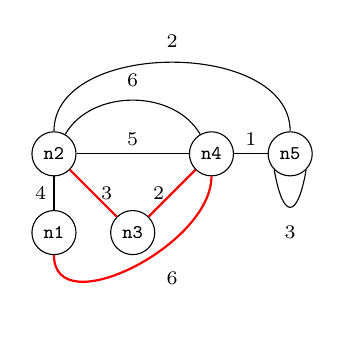
\begin{tikzpicture}[scale=1]\scriptsize
\node[draw,circle] (A) at (0,0) {\texttt{n1}};
\node[draw,circle] (B) at (0,1) {\texttt{n2}};
\node[draw,circle] (C) at (1,0) {\texttt{n3}};
\node[draw,circle] (D) at (2,1) {\texttt{n4}};
\node[draw,circle] (E) at (3,1) {\texttt{n5}};
\draw (A) -- (B);
\draw (0,0.5) node[left] {4};
\draw[thick,color=red] (B) -- (C);
\draw (0.5,0.5) node[right] {3};
\draw[thick,color=red] (A) to[out=-90,in=-90] (D);
\draw (B) to[out=60,in=120] (D);
\draw (B) -- (D);
\draw[thick,color=red] (C) -- (D);
\draw (1.5,0.5) node[left] {2};
\draw (1,1) node[above] {5};
\draw (1.5,-0.4) node[below] {6};
\draw (1,1.75) node[above] {6};
\draw (D) -- (E);
\draw (2.5,1) node[above] {1};
\draw (B) to[out=90,in=90] (E);
\draw (1.5,2.25) node[above] {2};
\coordinate[shift={(0mm,-1cm)}] (n) at (E.south);
\draw[rounded corners=30pt] (E.south west) -- (n) -- (E.south east);
\draw (3,0) node {3};
\end{tikzpicture}}
\end{minipage}

\begin{question}[« tout en un » : chemins dans un graphe]\label{question:suivants}\mbox{}
\begin{enumerate}
\item Définir la fonction \texttt{Chemin} qui teste si un chemin est bien un doublet
	\texttt{(distance,route)} où \texttt{distance} est un nombre et \texttt{route} une liste 
	non vide de n\oe uds.

\noindent\begin{minipage}[t]{6cm}\tt\footnotesize
\begin{Verbatim}
>>> Chemin((7,['n1','n2','n3']))
True
\end{Verbatim}
\end{minipage}
\hfill
\begin{minipage}[t]{6cm}\tt\footnotesize
\begin{Verbatim}
>>> Chemin((7,[]))
False
\end{Verbatim}
\end{minipage}
\vspace*{2mm}

\item Définir la fonction \texttt{extremite} qui retourne le dernier n\oe ud de la route
	(liste des n\oe uds) maintenue dans un \texttt{chemin}.

\noindent\begin{minipage}[t]{6cm}\tt\footnotesize
\begin{Verbatim}
>>> extremite((7,['n1','n2','n3']))
'n3'
\end{Verbatim}
\end{minipage}
\hfill
\begin{minipage}[t]{6cm}\tt\footnotesize
\begin{Verbatim}
>>> extremite((7,[]))
    assert Chemin(chemin)
AssertionError
\end{Verbatim}
\end{minipage}
\vspace*{2mm}

\item Définir la fonction \texttt{cheminsSuivants} qui retourne la liste
	des chemins possibles à partir du n\oe ud extrémité d'un \texttt{chemin}
	d'un \texttt{graphe} donné sans repasser par l'un des n\oe uds du \texttt{chemin}.

\noindent\begin{minipage}[t]{6cm}\tt\footnotesize
\begin{Verbatim}
>>> g = [('n1','n2',4),('n2','n3',3),\
         ('n1','n4',6),('n2','n4',5),\
         ('n2','n4',6)]
>>> cheminsSuivants((0,['n1']),g)
[(4, ['n1', 'n2']), (6, ['n1', 'n4'])]
>>> cheminsSuivants((6,['n1','n4']),g)
[(11, ['n1', 'n4', 'n2']), 
 (12, ['n1', 'n4', 'n2'])]
\end{Verbatim}
\end{minipage}
\hfill
\begin{minipage}[t]{6cm}\tt\footnotesize
\begin{Verbatim}
>>> cheminsSuivants((4,['n1','n2']),g)
[(7, ['n1', 'n2', 'n3']), 
 (9, ['n1', 'n2', 'n4']), 
 (10, ['n1', 'n2', 'n4'])]
>>> cheminsSuivants((7,['n1','n2','n3']),g)
[]
>>> cheminsSuivants((9,['n1','n2','n4']),g)
[]
\end{Verbatim}
\end{minipage}
\vspace*{2mm}

\end{enumerate}
\end{question}

%-------------------------------------------------------------------------
\subsubsection{Recherches de chemins dans un graphe}\label{subsec:recherches}
%-------------------------------------------------------------------------
Le principe de la recherche d'un chemin dans un graphe nécessite de stocker 
les chemins partiels déjà explorés dans un tableau afin de vérifier qu'on ne passe
pas deux fois par le même n\oe ud. On initialise le tableau avec le chemin \texttt{(0,['depart'])} : on est
situé sur le n\oe ud de départ et on ne s'est pas encore déplacé dans le graphe. 
A chaque étape, on choisit un élément de ce tableau et si l'extrémité du chemin ainsi choisi 
est le n\oe ud d'arrivée, alors ce chemin est une solution du problème.
Si l'extrémité du chemin ne correspond pas au n\oe ud d'arrivée, on remplace ce chemin par l'ensemble de ses successeurs dans le graphe (voir \texttt{cheminsSuivants} de la 
question \ref{question:suivants} précédente) et on recommence ainsi de suite jusqu'à ce que
le tableau de stockage soit vide.

Différentes méthodes peuvent être mises en \oe uvre selon la procédure utilisée pour
stocker, choisir et remplacer les chemins partiels dans le tableau de stockage. 
Dans ce qui suit, on distinguera trois méthodes : la recherche en profondeur
qui utilise une pile, 
la recherche en largeur qui utilise une file et la recherche du meilleur chemin
qui utilise une pile (ou une file) triée à chaque étape.

Pour tester les différents algorithmes de recherche, on utilisera le 
réseau routier ci-dessous.
\vspace*{2mm}

\noindent\begin{minipage}{5.25cm}
\setlength\unitlength{0.6cm}\footnotesize
\reseau
\end{minipage}
\hfill
\begin{minipage}{5cm}\footnotesize\tt
\begin{Verbatim}
graphe = [('s','d',4),
          ('s','a',3),
          ('d','e',2),
          ('d','a',5),
          ('a','b',4),
          ('b','c',4),
          ('b','e',5),
          ('e','f',4),
          ('f','g',3)]
\end{Verbatim}
\end{minipage}
\hfill\mbox{}
\vspace*{2mm}


\begin{question}[« tout en un » : recherche en profondeur]
La recherche en profondeur consiste à stocker les chemins dans une pile 
comme l'illustre la figure ci-dessous.
\vspace*{3mm}

\begin{center}\footnotesize
\setlength{\unitlength}{0.8cm}
\begin{picture}(14,6.5)
\multiput(0,4)(0,0.5){4}{\framebox(2.5,0.5){}}
\put(0,3.5){\makebox(2.5,0.5){1}}
%%\pause
\put(0,4){\makebox(2.5,0.5){\tt [s]}}
%\pause
\put(2,5.9){\line(0,1){0.6}}
\put(2,6.5){\vector(1,0){0.6}}
\put(3.25,6.5){\makebox(0,0.5){\color{orange}s $\stackrel{?}{=}$ g}}
%\pause
\put(4,3.5){\makebox(2.5,0.5){2}}
\multiput(4,4)(0,0.5){4}{\framebox(2.5,0.5){}}
\put(3.9,6.5){\line(1,0){0.6}}
\put(4.5,6.5){\vector(0,-1){0.6}}
%\pause
\put(4,4.5){\makebox(2.5,0.5){\tt [s,a]}}
\put(4,4){\makebox(2.5,0.5){\tt [s,d]}}
%\pause
\put(6,5.9){\line(0,1){0.6}}
\put(6,6.5){\vector(1,0){0.6}}
\put(7.25,6.5){\makebox(0,0.5){\color{orange}a $\stackrel{?}{=}$ g}}
%\pause
\put(8,3.5){\makebox(2.5,0.5){3}}
\multiput(8,4)(0,0.5){4}{\framebox(2.5,0.5){}}
\put(7.9,6.5){\line(1,0){0.6}}
\put(8.5,6.5){\vector(0,-1){0.6}}
\put(8,5){\makebox(2.5,0.5){\tt [s,a,b]}}
\put(8,4.5){\makebox(2.5,0.5){\tt [s,a,d]}}
\put(8,4){\makebox(2.5,0.5){\tt [s,d]}}
%\pause
\put(10,5.9){\line(0,1){0.6}}
\put(10,6.5){\vector(1,0){0.6}}
\put(11.25,6.5){\makebox(0,0.5){\color{orange}b $\stackrel{?}{=}$ g}}
%\pause
\put(12,3.5){\makebox(2.5,0.5){4}}
\multiput(12,4)(0,0.5){4}{\framebox(2.5,0.5){}}
\put(11.9,6.5){\line(1,0){0.6}}
\put(12.5,6.5){\vector(0,-1){0.6}}
\put(12,5.5){\makebox(2.5,0.5){\tt [s,a,b,c]}}
\put(12,5){\makebox(2.5,0.5){\tt [s,a,b,e]}}
\put(12,4.5){\makebox(2.5,0.5){\tt [s,a,d]}}
\put(12,4){\makebox(2.5,0.5){\tt [s,d]}}
%\pause
\put(14,5.9){\line(0,1){0.6}}
\put(14,6.5){\vector(1,0){0.6}}
\put(15.25,6.5){\makebox(0,0.5){\color{orange}c $\stackrel{?}{=}$ g}}
\put(-0.8,3){\makebox(0,0.5){\color{orange}c $\stackrel{?}{=}$ g}}
%\pause
\put(-0.1,3){\line(1,0){0.6}}
\put(0.5,3){\vector(0,-1){0.6}}
\multiput(0,0.5)(0,0.5){4}{\framebox(2.5,0.5){}}
\put(0,0){\makebox(2.5,0.5){5}}
\put(0,1.5){\makebox(2.5,0.5){\tt [s,a,b,e]}}
\put(0,1){\makebox(2.5,0.5){\tt [s,a,d]}}
\put(0,0.5){\makebox(2.5,0.5){\tt [s,d]}}
%\pause
\put(2,2.4){\line(0,1){0.6}}
\put(2,3){\vector(1,0){0.6}}
\put(3.25,3){\makebox(0,0.5){\color{orange}e $\stackrel{?}{=}$ g}}
%\pause
\put(3.9,3){\line(1,0){0.6}}
\put(4.5,3){\vector(0,-1){0.6}}
\multiput(4,0.5)(0,0.5){4}{\framebox(2.5,0.5){}}
\put(4,0){\makebox(2.5,0.5){6}}
\put(4,2){\makebox(2.5,0.5){\tt [s,a,b,e,d]}}
\put(4,1.5){\makebox(2.5,0.5){\tt [s,a,b,e,f]}}
\put(4,1){\makebox(2.5,0.5){\tt [s,a,d]}}
\put(4,0.5){\makebox(2.5,0.5){\tt [s,d]}}
%\pause
\put(6,2.4){\line(0,1){0.6}}
\put(6,3){\vector(1,0){0.6}}
\put(7.25,3){\makebox(0,0.5){\color{orange}d $\stackrel{?}{=}$ g}}
%\pause
\put(7.9,3){\line(1,0){0.6}}
\put(8.5,3){\vector(0,-1){0.6}}
\multiput(8,0.5)(0,0.5){4}{\framebox(2.5,0.5){}}
\put(8,0){\makebox(2.5,0.5){7}}
\put(8,1.5){\makebox(2.5,0.5){\tt [s,a,b,e,f]}}
\put(8,1){\makebox(2.5,0.5){\tt [s,a,d]}}
\put(8,0.5){\makebox(2.5,0.5){\tt [s,d]}}
%\pause
\put(10,2.4){\line(0,1){0.6}}
\put(10,3){\vector(1,0){0.6}}
\put(11.25,3){\makebox(0,0.5){\color{orange}f $\stackrel{?}{=}$ g}}
%\pause
\put(11.9,3){\line(1,0){0.6}}
\put(12.5,3){\vector(0,-1){0.6}}
\multiput(12,0.5)(0,0.5){4}{\framebox(2.5,0.5){}}
\put(12,0){\makebox(2.5,0.5){8}}
\put(12,1.5){\makebox(2.5,0.5){\tt [s,a,b,e,f,g]}}
\put(12,1){\makebox(2.5,0.5){\tt [s,a,d]}}
\put(12,0.5){\makebox(2.5,0.5){\tt [s,d]}}
%\pause
\put(14,2.4){\line(0,1){0.6}}
\put(14,3){\vector(1,0){0.6}}
\put(15.25,3){\makebox(0,0.5){\color{orange}g $\stackrel{?}{=}$ g}}
\end{picture}
\end{center}

\begin{enumerate}
\item Définir ainsi la fonction \texttt{profondeur} qui retourne la liste 
		de tous les chemins qui mènent d'un n\oe ud \texttt{depart} à un n\oe ud 
		\texttt{arrivee} dans un graphe \texttt{g}.

\noindent\begin{minipage}[t]{7cm}\tt\footnotesize
\begin{Verbatim}
>>> profondeur('s','g',graphe)
[(19, ['s', 'a', 'b', 'e', 'f', 'g']), 
 (17, ['s', 'a', 'd', 'e', 'f', 'g']), 
 (25, ['s', 'd', 'a', 'b', 'e', 'f', 'g']), 
 (13, ['s', 'd', 'e', 'f', 'g'])]
\end{Verbatim}
\end{minipage}
\hfill
\begin{minipage}[t]{7cm}\tt\footnotesize
\begin{Verbatim}
>>> profondeur('d','b',graphe)
[(9, ['d', 'a', 'b']), 
 (7, ['d', 'e', 'b']), 
 (11, ['d', 's', 'a', 'b'])]
\end{Verbatim}
\end{minipage}
\vspace*{2mm}
	
\item Justifier pourquoi cette méthode est appelée recherche en profondeur.
\end{enumerate}
\end{question}

\begin{question}[« tout en un » : recherche en largeur]
La recherche en largeur consiste à stocker les chemins dans une file 
comme l'illustre la figure ci-dessous.
\vspace*{5mm}

\begin{center}\footnotesize
\setlength{\unitlength}{0.8cm}
\begin{picture}(14.5,4.5)
\put(0,4.5){\makebox(0,0.5){1}}
\put(0.6,4.5){\makebox(0,0.5)[l]{$\longrightarrow$}}
\put(1,4.5){\framebox(2.5,0.5){\tt [s]}}
%\pause
\put(3.4,4.5){\makebox(0,0.5)[l]{$\longrightarrow$ \color{orange}\tt s $\stackrel{?}{=}$ g}}
%\pause
\put(0,3.75){\makebox(0,0.5){2}}
\put(0.6,3.75){\makebox(0,0.5)[l]{$\longrightarrow$}}
\put(1,3.75){\framebox(2.5,0.5){\tt [s,d]}}
\put(3.5,3.75){\framebox(2.5,0.5){\tt [s,a]}}
%\pause
\put(5.9,3.75){\makebox(0,0.5)[l]{$\longrightarrow$ \color{orange}\tt a $\stackrel{?}{=}$ g}}
%\pause
\put(0,3){\makebox(0,0.5){3}}
\put(0.6,3){\makebox(0,0.5)[l]{$\longrightarrow$}}
\put(1,3){\framebox(2.5,0.5){\tt [s,a,d]}}
\put(3.5,3){\framebox(2.5,0.5){\tt [s,a,b]}}
\put(6,3){\framebox(2.5,0.5){\tt [s,d]}}
%\pause
\put(8.4,3){\makebox(0,0.5)[l]{$\longrightarrow$ \color{orange}\tt d $\stackrel{?}{=}$ g}}
%\pause
\put(0,2.25){\makebox(0,0.5){4}}
\put(0.6,2.25){\makebox(0,0.5)[l]{$\longrightarrow$}}
\put(1,2.25){\framebox(2.5,0.5){\tt [s,d,e]}}
\put(3.5,2.25){\framebox(2.5,0.5){\tt [s,d,a]}}
\put(6,2.25){\framebox(2.5,0.5){\tt [s,a,d]}}
\put(8.5,2.25){\framebox(2.5,0.5){\tt [s,a,b]}}
%\pause
\put(10.9,2.25){\makebox(0,0.5)[l]{$\longrightarrow$ \color{orange}\tt b $\stackrel{?}{=}$ g}}
%\pause
\put(0,1.5){\makebox(0,0.5){$\vdots$}}
%\pause
\put(0,0.75){\makebox(0,0.5){22}}
\put(1,0.75){\framebox(2.5,0.5){\tt [s,d,a,b,e,f]}}
\put(3.5,0.75){\dashbox(2.5,0.5){\tt \ldots}}
\put(6,0.75){\framebox(2.5,0.5){\tt [s,d,e,f,g]}}
%\pause
\put(8.4,0.75){\makebox(0,0.5)[l]{$\longrightarrow$ \color{orange}\tt g $\stackrel{?}{=}$ g}}
\end{picture}
\end{center}

\begin{enumerate}
\item Définir ainsi la fonction \texttt{largeur} qui retourne la liste de 
		tous les chemins qui mènent d'un n\oe ud \texttt{depart} à un n\oe ud 
		\texttt{arrivee} dans un graphe	\texttt{g}.

\noindent\begin{minipage}[t]{7cm}\tt\footnotesize
\begin{Verbatim}
>>> largeur('s','g',graphe)
[(13, ['s', 'd', 'e', 'f', 'g']), 
 (19, ['s', 'a', 'b', 'e', 'f', 'g']), 
 (17, ['s', 'a', 'd', 'e', 'f', 'g']), 
 (25, ['s', 'd', 'a', 'b', 'e', 'f', 'g'])]
\end{Verbatim}
\end{minipage}
\hfill
\begin{minipage}[t]{7cm}\tt\footnotesize
\begin{Verbatim}
>>> largeur('d','b',graphe)
[(9, ['d', 'a', 'b']), 
 (7, ['d', 'e', 'b']), 
 (11, ['d', 's', 'a', 'b'])]
\end{Verbatim}
\end{minipage}
\vspace*{2mm}

\item Justifier pourquoi cette méthode est appelée recherche en largeur.
\end{enumerate}
\end{question}

\begin{question}[« tout en un » : recherche du meilleur chemin]
La recherche du meilleur chemin consiste à stocker les chemins dans une pile 
	(ou file) et à trier cette pile (ou file) à chaque
	étape.
\begin{enumerate}
\item Définir ainsi la fonction \texttt{meilleur} qui retourne la liste 
		de tous les chemins qui mènent d'un n\oe ud \texttt{depart} à un 
		n\oe ud \texttt{arrivee} dans un graphe	\texttt{g}.

\noindent\begin{minipage}[t]{7cm}\tt\footnotesize
\begin{Verbatim}
>>> meilleur('s','g',graphe)
[(13, ['s', 'd', 'e', 'f', 'g']), 
 (17, ['s', 'a', 'd', 'e', 'f', 'g']), 
 (19, ['s', 'a', 'b', 'e', 'f', 'g']), 
 (25, ['s', 'd', 'a', 'b', 'e', 'f', 'g'])]
\end{Verbatim}
\end{minipage}
\hfill
\begin{minipage}[t]{7cm}\tt\footnotesize
\begin{Verbatim}
>>> meilleur('d','b',graphe)
[(7, ['d', 'e', 'b']), 
 (9, ['d', 'a', 'b']), 
 (11, ['d', 's', 'a', 'b'])]
\end{Verbatim}
\end{minipage}
\vspace*{2mm}

\item Justifier pourquoi cette méthode garantit que les chemins sont obtenus
		par ordre croissant de la distance parcourue.
\end{enumerate}

\end{question}

%-------------------------------------------------------------------------
\subsection{Généralisation}
%-------------------------------------------------------------------------

\noindent
\begin{minipage}{7.5cm}
Soit un système dans un état initial donné. On veut le faire passer
dans un état final donné connaissant les opérations élémentaires 
que l'on peut appliquer sur le système.
Quelle(s) suite(s) d'opérations élémentaires doit-on appliquer 
au système pour le faire passer de l'état initial à l'état 
final ?
\end{minipage}
\hfill
\begin{minipage}{7.5cm}
\begin{center}
\setlength{\unitlength}{0.6cm}
\begin{picture}(12,5)
\put(2.5,2.5){\oval(5,5)}
%\multiput(2.5,2.5)(7,0){2}{\oval(5,5)}
\put(2.5,2.5){\makebox(0,1){\bf \'etat}}
\put(2.5,1.5){\makebox(0,1){\bf initial}}
\put(9.5,2.5){\oval(5,5)}
\put(5.5,2.5){\color{orange}\vector(1,0){1}}
\put(6,2.5){\makebox(0,1){\color{orange}\bf ?}}
\put(9.5,2.5){\makebox(0,1){\bf \'etat}}
\put(9.5,1.5){\makebox(0,1){\bf final}}
\end{picture}
\end{center}
\end{minipage}
\vspace*{2mm}

Dans le cas du réseau routier de la section \ref{subsec:recherches} précédente, 
l'état initial est simplement le fait d'être en \texttt{s} et l'état final d'être 
en \texttt{g}. La seule opération élémentaire consiste à suivre une route
qui part de la ville où l'on se trouve. Dans le cas d'un réseau routier réel,
on imagine aisément que le nombre de possibilités pour aller d'une ville à une
autre est considérable et qu'en conséquence l'arbre de recherche des solutions
est immense : on parle alors d'« explosion combinatoire ».


\begin{question}[« tout en un » : une ou plusieurs solutions] Modifier les fonctions
\texttt{profondeur}, \linebreak\texttt{largeur} et \texttt{meilleur} précédentes de telle
manière qu'elles ne retournent qu'un nombre \texttt{n} maximum de solutions.

\noindent\begin{minipage}[t]{7cm}\tt\footnotesize
\begin{Verbatim}
>>> meilleur('s','g',graphe,10)
[(13, ['s', 'd', 'e', 'f', 'g']), 
 (17, ['s', 'a', 'd', 'e', 'f', 'g']), 
 (19, ['s', 'a', 'b', 'e', 'f', 'g']), 
 (25, ['s', 'd', 'a', 'b', 'e', 'f', 'g'])]
\end{Verbatim}
\end{minipage}
\hfill
\begin{minipage}[t]{7cm}\tt\footnotesize
\begin{Verbatim}
>>> meilleur('s','g',graphe,1)
[(13, ['s', 'd', 'e', 'f', 'g'])]
>>> meilleur('s','g',graphe,2)
[(13, ['s', 'd', 'e', 'f', 'g']), 
 (17, ['s', 'a', 'd', 'e', 'f', 'g'])]
\end{Verbatim}
\end{minipage}
\vspace*{2mm}

\end{question}

Toujours dans le cas d'un réseau routier, le graphe du réseau est explicite : 
il est connu à l'avance et on peut ainsi le « passer » à la fonction de recherche. 
Mais il existe des problèmes où ce n'est pas le cas : il suffit de penser au 
« Rubik's cube » et ses 43 trillions (milliards de milliards : $10^{18}$) de 
combinaisons possibles ! Dans ces cas là, plutôt que de passer explicitement 
le graphe à la fonction de recherche, on lui transmet la fonction qui, à partir 
d'un n\oe ud donné, applique les différentes opérations élémentaires autorisées
pour obtenir les n\oe uds adjacents et ainsi construire le graphe au fur et à 
mesure des étapes.

\begin{question}[« tout en un » : explicite versus implicite] \mbox{}
\begin{enumerate}
\item Définir la fonction \texttt{reseau} qui retourne les arcs issus d'un n\oe ud
	du réseau routier de la section \ref{subsec:recherches} précédente.
	
\noindent\begin{minipage}[t]{7cm}\tt\footnotesize
\begin{Verbatim}
>>> reseau('a')
[('s', 'a', 3), 
 ('d', 'a', 5), 
 ('a', 'b', 4)]
\end{Verbatim}
\end{minipage}
\hfill
\begin{minipage}[t]{7cm}\tt\footnotesize
\begin{Verbatim}
>>> reseau('s')
[('s', 'd', 4), ('s', 'a', 3)]
>>> reseau('c')
[('b', 'c', 4)]
\end{Verbatim}
\end{minipage}
\vspace*{2mm}

\item Modifier les fonctions
\texttt{profondeur}, \texttt{largeur} et \texttt{meilleur} précédentes afin 
de leur transmettre la fonction \texttt{f} qui retourne les arcs issus d'un n\oe ud donné.

\noindent\begin{minipage}[t]{7cm}\tt\footnotesize
\begin{Verbatim}
>>> meilleur('s','g',reseau,1)
[(13, ['s', 'd', 'e', 'f', 'g'])]
\end{Verbatim}
\end{minipage}
\hfill
\begin{minipage}[t]{7cm}\tt\footnotesize
\begin{Verbatim}
>>> meilleur('d','b',reseau,1)
[(7, ['d', 'e', 'b'])]
\end{Verbatim}
\end{minipage}
\vspace*{2mm}

\end{enumerate}


\end{question}

%-------------------------------------------------------------------------
\subsection{Applications}
%-------------------------------------------------------------------------

\begin{question}[« tout en un » : vases]
Soit un système composé de deux récipients non gradués $R_1$ et $R_2$, 
	respectivement de capacité $C_1$ et $C_2$. L'état du système sera représenté
	par la paire $(V_1,V_2)$ caractérisant la quantité d'eau contenue dans chacun
	des récipients. On veut faire passer le système de l'état initial $(V_1^i,V_2^i)$
	à l'état final $(V_1^f,V_2^f)$ sachant que les seules opérations élémentaires 
	autorisées sont :
	remplir complètement un récipient,
	vider complètement un récipient
	ou transvaser un récipient dans l'autre sans perdre une seule goutte.
	Pour fixer les idées, on prendra $C_1 = 8l$, $C_2 = 5l$, $V_1^i = V_2^i = 0l$,
	$V_1^f = 4l$ et $V_2^f = 0l$.
\vspace*{2mm}

\noindent
\begin{minipage}{7.5cm}
\begin{enumerate}
\item Définir la fonction \texttt{vases} qui applique les opérations élémentaires
	possibles (vider, remplir, transvaser) à un état donné \texttt{(v1,v2)}.
\item Trouver les 5 meilleures suites d'opérations élémentaires
	pour passer de l'état \texttt{(0,0)} à l'état \texttt{(4,0)}.
\end{enumerate}
\end{minipage}
\hfill
\begin{minipage}{7.5cm}
\setlength{\unitlength}{0.6cm}\footnotesize
\begin{picture}(12,6)
\put(1,5){\oval(2,8)[b]}
\put(1,5){\makebox(0,1){$C_1 = 8\,l$}}
\put(1,0){\makebox(0,1){$V_1 = 0\,l$}}
\put(4,3.5){\oval(2,5)[b]}
\put(4,3.5){\makebox(0,1){$C_2 = 5\,l$}}
\put(4,0){\makebox(0,1){$V_2 = 0\,l$}}
\put(8,5){\oval(2,8)[b]}
\put(8,5){\makebox(0,1){$C_1 = 8\,l$}}
\put(8,0){\makebox(0,1){$V_1 = 4\,l$}}
\put(7,3.2){\line(1,0){2}}
\put(11,3.5){\oval(2,5)[b]}
\put(11,3.5){\makebox(0,1){$C_2 = 5\,l$}}
\put(11,0){\makebox(0,1){$V_2 = 0\,l$}}
\put(5.5,2.5){\color{orange}\vector(1,0){1}}
\put(6,2.5){\makebox(0,0.8){\color{orange}\bf ?}}
\end{picture}
\end{minipage}
\vspace*{2mm}

\noindent\begin{minipage}{\textwidth}\em\footnotesize
\begin{Verbatim}
>>> vases((0,0))
[((0, 0), (0, 5), 1), ((0, 0), (8, 0), 1)]
>>> vases((8,0))
[((8, 0), (3, 5), 1), ((8, 0), (8, 5), 1), ((8, 0), (0, 0), 1)]
>>> vases((0,5))
[((0, 5), (5, 0), 1), ((0, 5), (8, 5), 1), ((0, 5), (0, 0), 1)]

>>> meilleur((0,0),(4,0),vases,5)
[(12, [(0, 0), (0, 5), (5, 0), (5, 5), (8, 2), (0, 2), (2, 0), (2, 5), (7, 0), (7, 5), (8, 4),
       (0, 4), (4, 0)]), 
 (13, [(0, 0), (8, 0), (3, 5), (3, 0), (0, 3), (8, 3), (6, 5), (6, 0), (1, 5), (1, 0), (0, 1), 
       (8, 1), (4, 5), (4, 0)]), 
 (14, [(0, 0), (8, 0), (3, 5), (0, 5), (5, 0), (5, 5), (8, 2), (0, 2), (2, 0), (2, 5), (7, 0),
       (7, 5), (8, 4), (0, 4), (4, 0)]), 
 (14, [(0, 0), (8, 0), (8, 5), (0, 5), (5, 0), (5, 5), (8, 2), (0, 2), (2, 0), (2, 5), (7, 0),
       (7, 5), (8, 4), (0, 4), (4, 0)]), 
 (15, [(0, 0), (0, 5), (5, 0), (8, 0), (3, 5), (3, 0), (0, 3), (8, 3), (6, 5), (6, 0), (1, 5),
       (1, 0), (0, 1), (8, 1), (4, 5), (4, 0)])]
\end{Verbatim}
\end{minipage}

\end{question}

\begin{question}[« tout en un » : taquin] Le taquin est un jeu en forme de damier $(n\times n)$.
Il est composé de $(n^2 - 1)$ petits carreaux numérotés de 1 à $(n^2 - 1)$ qui glissent dans un cadre prévu pour $n^2$ carreaux. Il consiste à remettre dans l'ordre les $(n^2 - 1)$ carreaux à partir d'une configuration initiale quelconque.

\noindent
\begin{minipage}{5.575cm}\em
\setlength{\unitlength}{0.6cm}
\begin{picture}(9,5)
\put(0,1){\framebox(3,3){}} 
\put(0.1,1.1){\framebox(0.8,0.8){7}}
\put(1.1,1.1){\framebox(0.8,0.8){5}}
\put(2.1,2.1){\framebox(0.8,0.8){3}}
\put(2.1,1.1){\framebox(0.8,0.8){4}}
\put(2.1,3.1){\framebox(0.8,0.8){8}}
\put(1.1,3.1){\framebox(0.8,0.8){1}}
\put(0.1,3.1){\framebox(0.8,0.8){2}}
\put(0.1,2.1){\framebox(0.8,0.8){6}}
\put(6,1){\framebox(3,3){}} 
\put(6.1,1.1){\framebox(0.8,0.8){7}}
\put(7.1,1.1){\framebox(0.8,0.8){8}}
\put(6.1,2.1){\framebox(0.8,0.8){4}}
\put(7.1,2.1){\framebox(0.8,0.8){5}}
\put(8.1,2.1){\framebox(0.8,0.8){6}}
\put(6.1,3.1){\framebox(0.8,0.8){1}}
\put(7.1,3.1){\framebox(0.8,0.8){2}}
\put(8.1,3.1){\framebox(0.8,0.8){3}}
\put(3.5,2.5){\color{orange}\vector(1,0){2}}
\put(4.5,2.5){\makebox(0,1){\color{orange}\bf ?}}
\put(4.5,0.15){\makebox(0,0){taquin $(3\times 3)$}}
\end{picture}
\end{minipage}
\hfill
\begin{minipage}{8.5cm}\em
Le carreau vide est numéroté \texttt{0} :
$$\begin{tabular}{lll}
état initial 	&:& \texttt{[[2,1,8],[6,0,3],[7,5,4]]}\\ 
\color{orange}$\downarrow$ ?   & & \\
état final 		&:& \texttt{[[1,2,3],[4,5,6],[7,8,0]]}
\end{tabular}$$
\end{minipage}

\begin{enumerate}
\item Définir la fonction \texttt{taquin} qui applique les opérations élémentaires
	possibles à partir d'une configuration donnée pour un damier $(n\times n)$.
	\vspace*{0.2mm}
	
\noindent\begin{minipage}{\textwidth}\em\footnotesize
\begin{Verbatim}
>>> jeu  = [[3,1],[0,2]]
>>> taquin(jeu)
[([[3, 1], [0, 2]], [[0, 1], [3, 2]], 1), 
 ([[3, 1], [0, 2]], [[3, 1], [2, 0]], 1)]
 
>>> jeu  = [[2,1,8],[6,0,3],[7,5,4]]
>>> taquin(jeu)
[([[2, 1, 8], [6, 0, 3], [7, 5, 4]], [[2, 0, 8], [6, 1, 3], [7, 5, 4]], 1), 
 ([[2, 1, 8], [6, 0, 3], [7, 5, 4]], [[2, 1, 8], [6, 5, 3], [7, 0, 4]], 1), 
 ([[2, 1, 8], [6, 0, 3], [7, 5, 4]], [[2, 1, 8], [0, 6, 3], [7, 5, 4]], 1), 
 ([[2, 1, 8], [6, 0, 3], [7, 5, 4]], [[2, 1, 8], [6, 3, 0], [7, 5, 4]], 1)]
\end{Verbatim}
\end{minipage}

\item Trouver la  meilleure suite d'opérations élémentaires
	pour passer de l'état \texttt{[[3,1],[0,2]]} à l'état 
	\texttt{[[1,2],[3,0]]} dans un taquin $(2\times 2)$.
	\vspace*{0.2mm}
	
\noindent\begin{minipage}{\textwidth}\em\footnotesize
\begin{Verbatim}
>>> depart  = [[3,1],[0,2]]
>>> arrivee = [[1,2],[3,0]]
>>> meilleur(depart,arrivee,taquin,10)
[(3, [[[3, 1], [0, 2]], [[0, 1], [3, 2]], [[1, 0], [3, 2]], [[1, 2], [3, 0]]]), 
 (9, [[[3, 1], [0, 2]], [[3, 1], [2, 0]], [[3, 0], [2, 1]], [[0, 3], [2, 1]], 
      [[2, 3], [0, 1]], [[2, 3], [1, 0]], [[2, 0], [1, 3]], [[0, 2], [1, 3]], 
      [[1, 2], [0, 3]], [[1, 2], [3, 0]]])]
\end{Verbatim}
\end{minipage}

\item Trouver la  meilleure suite d'opérations élémentaires
	pour passer de l'état \texttt{[[2,1,8],[6,0, 3], [7,5,4]]} à l'état 
	\texttt{[[1,2,3],[4,5,6],[7,8,0]]} dans un taquin $(3\times 3)$.
	\vspace*{0.2mm}

\noindent\begin{minipage}{\textwidth}\em\footnotesize
\begin{Verbatim}
>>> depart  = [[2,1,8],[6,0,3],[7,5,4]]
>>> arrivee = [[1,2,3],[4,5,6],[7,8,0]]
>>> meilleur(depart,arrivee,taquin,1)
...
\end{Verbatim}
\end{minipage}

\end{enumerate}

\end{question}

Ce dernier exemple, qui n'en finit pas de calculer, du taquin $(3\times 3)$ illustre clairement le problème évoqué plus haut
de l'« explosion combinatoire ». Il révèle ainsi la limite des stratégies de recherche
développées ici (profondeur, largeur, meilleur chemin). 
Il faudrait en effet envisager de nouvelles stratégies, moins « aveugles » et mieux « informées » du problème considéré. Mais l'étude de telles stratégies dépasse
largement la cadre d'une simple initiation à l'algorithmique.
